\section{Data Visualization}
\begin{itemize}
    \item See trends, clusters and patterns in data
    \item Difficult to see in raw data
    \item Detect outliers and unusual groups
    \item Validate Hypothesis/Conjecture/Theory
\end{itemize}
\textbf{Important in a Plot:}
\begin{itemize}
    \item X-Axis / Y-Axis
    \item Title
    \item Scale
    \item Dimensionality of the data 2D / 3D
\end{itemize}
%\textbf{Plot types:}
%\begin{itemize}
%    \item \textit{Line}: trends, movement over time
%    \item \textit{Bar}: categorical data where binning/counting is done
%    \item \textit{Histogram (Häufigkeitsverteilung)}: represents the empirical distribution. number of observations vs bins (range of values)
%    \item \textit{Box \& Violin}: Descriptive Statistics (empirische Daten/Sammlung von Daten durch Tabellen, Kennzahlen und Grafiken übersichtlich darzustellen)
%    \item \textit{Scatter (Punktewolke)}: relationship between two continuous variables. color to encode a third variable
%\end{itemize}

\subsection{Descriptive statistics (Mittelwerte für Boxplots, etc.)}
\textbf{Mean (Normalfall)}
\begin{itemize}
    \item ''normaler'' Durchschnitt
    \item ist stark von Abreissern abhängig resp. Ausreisser verändern Auswertung sehr stark
\end{itemize}
\textbf{Median}
\begin{itemize}
    \item Der Wert, der genau in der Mitte einer Datenverteilung liegt (Bei 10 Punkten ist 5. Punkt der Median)
    \item ist nicht gross abhängig von Ausreissern und kann somit ein genaueres/ repräsentativeres Ergebnis darstellen
    \item wenn Daten Tendenz in eine Richtung haben (damit Ergebnis Aussagekräftig bleibt)
\end{itemize}
\textbf{Percentile}
\begin{itemize}
    \item wird verwendet, wenn andere Werte als die zentralen Werte der Daten gefunden werden müssen \item Während bei der Verwendung des Medians die Daten in zwei gleiche Hälften geteilt werden und der mittlere Wert berechnet wird, bietet die Perzentilmethode die Flexibilität, jeden beliebigen Wert zu berechnen, wenn die Daten zwischen 1 und 100 geteilt werden. 
\end{itemize}
\textbf{Häufig genutzte Percentile}
\begin{itemize}
    \item 50\%-Percentile = Median
    \item 25\%-Percentile = 1. Quantil
    \item 75\%-Percentile = 3. Quantil
\end{itemize}

\subsection{Data Analysis Libraries}
\subsubsection{NumPy}
\begin{itemize}
    \item Package for scientific computing in Python
    \item Multidimensional array object
    \item Routines for fast array operations (sorting, selecting, FFT, linalg, etc)
\end{itemize}

\subsubsection{pandas}
\begin{itemize}
    \item Built on top of NumPy
    \item Routines for accessing tabular data from files (.csv, xls, etc.)
    \item Supports 2-dimensional data (dataframe and series)
    \item Dataframes are something like database tables
\end{itemize}

\subsubsection{MatPlotLib}
\begin{itemize}
    \item Library for visualizing data
    \item Bargraphs, Histograms, Piecharts, Scatter plots, lines, boxplots, heatmaps, etc.
\end{itemize}

\subsubsection{Seaborn}
\begin{itemize}
    \item Extension of MatPlotLib, NumPy and pandas
    \item More user friendly
    \item Plots are aesthetically better
\end{itemize}

\subsubsection{Chart types}
\textbf{Line Plots}
\begin{itemize}
    \item \textit{Bivariate, Continous}
    \item Recognizes trend (pattern of change)
    \item general movement over time of a statistically detectable change
\end{itemize}
\textbf{Bar Chart}
\begin{itemize}
    \item Used for \textit{categorical data}
    \item Counting based on each category (e.g. Apps in AppStore, PlayStore, Windows Store, etc.)
\end{itemize}
\textbf{Histogram (Häufigkeitsverteilung)}
\begin{itemize}
    \item Represents the \textit{empirical distribution} of a variable
    \item Automatically creates bins (interval) along the range of values
    \item Shows vertical bars to indicate the number of observations / bin
\end{itemize}
\textbf{Descriptive Statistics: Box Plots and Violin Plots}\\
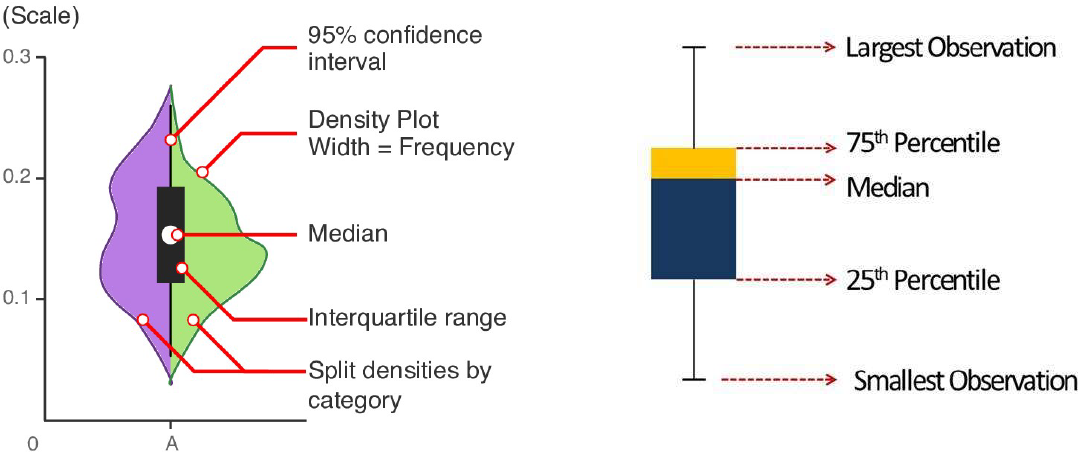
\includegraphics[width=\linewidth]{./img/descriptive_statistics.png}
\textbf{Scatter Plot}
\begin{itemize}
    \item Relationship between two \textit{continous} variables
    \item Helps to get an idea of the degree of correlation between variables
\end{itemize}